% Software and Tools used
\chapter{Εργαλεία Λογισμικού}
\label{chapter:tools}

Στο κεφάλαιο αυτό παρουσιάζονται τα εργαλεία λογισμικού που χρησιμοποιήθηκαν, τόσο για τις υλοποιήσεις όσο και για τα περάματα, που περιγράφονται στο \autoref{chapter:implementations} και  \autoref{chapter:experiments} αντίστοιχα. Επιπλέον, αξίζει να σημειωθεί ότι κύριο εργαλείο των υλοποιήσεων αλλά και των εργαλείων που χρησιμοποιήθηκαν είναι η γλώσσα προγραμματισμού \emph{Python}\footnote{\url{https://www.python.org/}}.

\section{RASA framework}
\label{sec:rasa}
Το \emph{RASA}\footnote{\url{https://rasa.com/docs/rasa/}} είναι ένα εργαλείο ανοιχτού λογισμικού το οποίο χρησιμοποιείται για την ανάπτυξη ψηφιακών βοηθών. Πιο συγκεκριμένα, είναι υπεύθυνο για την κατανόηση κειμένου (συνήθως συζητήσεων) και την αυτοματοποιημένη παραγωγή κειμένου και φωνής. Η κατανόηση του κειμένου πραγματοποιείται μέσω της αναγνώρισης επιθυμιών (\emph{intents}) αλλά και οντοτήτων (\emph{entities}) στο κείμενο εισόδου. Τα \emph{intents} είναι οτιδήποτε προσπαθεί ο εκάστοτε χρήστης του συστήματος να επιτύχει, για παράδειγμα έναν χαιρετισμό, μία ερώτηση, τον προσδιορισμό μιας τοποθεσίας και άλλα. Τα \emph{entities} είναι λέξεις-κλειδιά που εξάγονται από το κείμενο και ενδέχεται να δείχνουν αριθμούς τηλεφώνου, το όνομα κάποιου, μία τοποθεσία, χρηματικά ποσά και άλλα. 

Από τα πιο σημαντικά κομμάτια ενός ψηφιακού βοηθού είναι να προβαίνει σε κάποια ενέργεια (\emph{action}) ανάλογα με την επιθυμία του χρήστη. Αυτή ακριβώς τη λειτουργικότητα παρέχει ο \emph{action server}. Για κάθε αίτημα, ο \emph{server}, έχοντας την πληροφορία της επιθυμίας και των εξαγόμενων οντοτήτων, εκτελεί το αντίστοιχο κομμάτι κώδικα και επιστρέφει την απάντηση στον ψηφιακό βοηθό. Η επικοινωνία του ψηφιακού βοηθού με τον \emph{server} πραγματοποιείται μέσω REpresentational State Transfer Application Programming Interface - \emph{REST APIs}\footnote{\url{https://restfulapi.net/}}.

Η μεγαλύτερη πρόκληση στη δημιουργία και τη συντήρηση των ψηφιακών βοηθών αποτελεί το γεγονός ότι είναι απίθανη η πρόβλεψη όλων των εισόδων του χρήστη στο σύστημα. Σε κάθε συνομιλία οι χρήστες διατυπώνουν ακριβώς αυτό που επιθυμούν. Ο βοηθός εκπαιδεύεται σε ένα σύνολο προκαθορισμένων συνομιλιών, στις οποίες καλείται να ανταποκριθεί. Οι συνομιλίες αυτές ορίζουν το σύνολο των χαρούμενων μονοπατιών (\emph{happy paths}), δηλαδή συνομιλίες που ο ψηφιακός βοηθός αναμένεται να διαχειριστεί. Έτσι, αφού εκπαιδευτεί ένας ψηφιακός βοηθός που είναι θέση να χειριστεί τα περισσότερα \emph{happy paths}, τότε χρησιμοποιείται το \emph{RASA-X}\footnote{\url{https://rasa.com/docs/rasa-x/}} για τη βελτίωση του βοηθού. Ωστόσο, μία συνομιλία ενδέχεται να ακολουθήσει διαφορετικά βήματα από αυτά που αναμένει ο ψηφιακός βοηθός, τα οποία ονομάζονται \emph{un-happy paths}. Το \emph{RASA-X} είναι ένα εργαλείο κλειστού λογισμικού το οποίο χρησιμοποιείται για ανάπτυξη βοηθών τροφοδοτούμενη από συνομιλίες (\emph{Conversation-Driven Development}), δηλαδή της διαδικασίας παρακολούθησης των συζητήσεων των χρηστών, την αξιολόγηση και την αξιοποίηση τους για την βελτιστοποίηση του ψηφιακού βοηθού. 



\section{Haystack open-source framework}
\label{sec:haystack}
Το \emph{Haystack}\footnote{\url{https://haystack.deepset.ai/overview/intro}} αποτελεί ένα \emph{open-source framework} για την κατασκευή συστημάτων αναζήτησης σε μεγάλο αριθμό εγγράφων. Οι πρόσφατες εξελίξεις στον τομέα της επεξεργασίας φυσικής γλώσσας έδωσαν την δυνατότητα για ανάπτυξη συστημάτων ερωτοαπαντήσεων, ανάκτηση και περίληψη κειμένου και το \emph{Haystack} αποτελεί τη γέφυρα μεταξύ της έρευνας και της υλοποίησης σε πραγματικά συστήματα.

Μερικά από τα κύρια πλεονεκτήματα του είναι η χρήση \emph{NLP} για αναζήτηση χρησιμοποιώντας μοντέλα τελευταίας τεχνολογίας (\emph{state of the art}) από δημοφιλής βιβλιοθήκες όπως το \emph{huggingface}\footnote{\url{https://huggingface.co/}}. Επιπλέον, υποστηρίζει πληθώρα βάσεων δεδομένων ανάμεσα στις οποίες είναι οι \emph{Elasticsearch, Milvus\footnote{\url{https://milvus.io/}}, FAISS\footnote{\url{https://ai.facebook.com/tools/faiss/}}, SQL\footnote{\url{https://www.mysql.com/}}} και άλλες. Τέλος, παρέχει εργαλεία για τη δημιουργία παραδειγμάτων, συλλογή σχολίων χρηστών, αξιολόγηση και \emph{finetuning} μοντέλων. 

Στο \autoref{fig:haystack_concepts} παρουσιάζεται η συνολική δομή ενός συστήματος του \emph{Haystack}. Τα έγγραφα πρώτα δέχονται προ-επεξεργασία, για την πιο αποδοτική αναζήτηση στη βάση δεδομένων, και έπειτα αποθηκεύονται σε αυτή. Από τα πιο σημαντικά κομμάτια του \emph{Haystack} είναι ο \emph{Retriever} και ο \emph{Reader}. Ο \emph{Retriever}, είναι κόμβος ο οποίος λειτουργεί σαν ένα φίλτρο το οποίο ανατρέχει όλα τα έγγραφα που είναι αποθηκευμένα στη βάση δεδομένων και αναζητά εκείνα τα έγγραφα που μοιάζουν πιο πολύ με την εισερχόμενη ερώτηση. Συνήθως χρησιμοποιείται σε συνδυασμό με τον \emph{Reader} ο οποίος είναι υπεύθυνος να ανατρέξει τα υποψήφια έγγραφα που επέστρεψε ο \emph{Retriever} και να επιστρέψει τις απαντήσεις στις εισόδους του συστήματος. Πρακτικά, εδώ ενσωματώνεται το NLP μοντέλο που θα χρησιμοποιηθεί για να αναζητήσει την απάντηση στα έγγραφα που επιστράφηκαν από τον \emph{Retriever}.

\begin{figure}[!ht]
  \centering
  \captionsetup{justification=centering}
  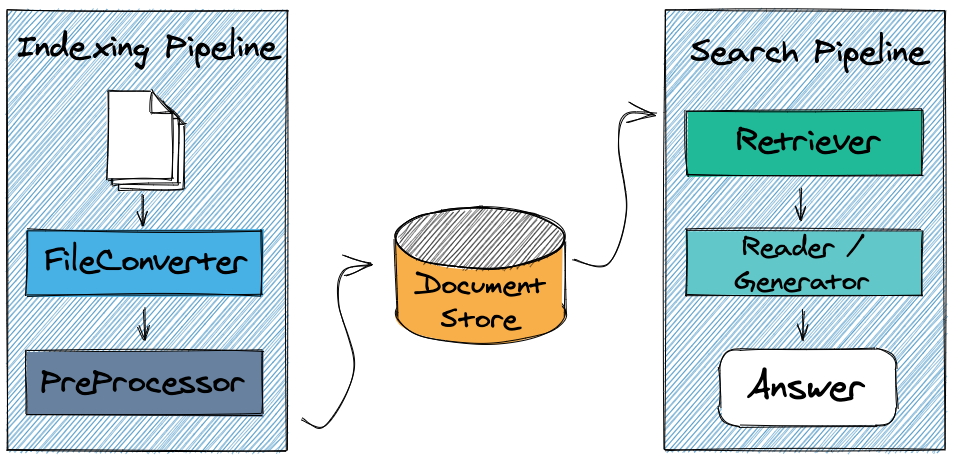
\includegraphics[width=0.7\textwidth]{images/chapter3/concepts_haystack_handdrawn.png}
  \captionsource{Βασική δομή \emph{Haystack}}{\url{https://haystack.deepset.ai/overview/intro}}
  \label{fig:haystack_concepts}
\end{figure}
\noindent

\section{Elasticsearch Database}
\label{sec:elastic}
Η \emph{Elasticsearch}\footnote{\url{https://www.elastic.co/}} είναι μία κατανεμημένη (\emph{distributed}) ανοιχτή μηχανή αναζήτησης και ανάλυσης για διάφορους τύπους δεδομένων, δομημένων ή μη, συμπεριλαμβανομένων κειμένων, αριθμητικών και γεωχωρικών. Είναι κυρίως γνωστή για την κατανεμημένη φύση, την ταχύτητα και την επεκτασιμότητα της και για τα απλά \emph{REST API} της. Επιπλέον, η αρχιτεκτονική της είναι βασισμένη στο \emph{Apache Lucene}\footnote{\url{https://lucene.apache.org/}} μιας βιβλιοθήκης ανοιχτού λογισμικού για την ανάπτυξη μηχανών αναζήτησης. 

\section{Beautiful Soup}
\label{sec:soup}
Το \emph{Beautiful Soup}\footnote{\url{https://beautiful-soup-4.readthedocs.io/en/latest/}} είναι μία βιβλιοθήκη της \emph{Python} η οποία χρησιμοποιείται για την επεξεργασία και την αναζήτηση σε έγγραφα \emph{HTML} και \emph{XML}. Τέτοιου είδους αρχεία συνήθως συναντώνται σε πηγαίους κώδικες ιστοσελίδων, κάνοντας έτσι πιο απλή την διαδικασία αυτοματοποιημένης εξαγωγής πληροφορίας από κείμενο που θα ήταν δύσκολο για έναν απλό χρήστη.

\section{Docker \& Kubernetes}
\label{sec:docker-kubernetes}
Το \emph{Docker}\footnote{\url{https://www.docker.com/}} είναι μία ανοιχτή πλατφόρμα για ανάπτυξη και εκτέλεση εφαρμογών και δίνει τη δυνατότητα διαχωρισμού της εφαρμογής που εκτελείται από το υπόλοιπο σύστημα. Αυτό επιτυγχάνεται με τη χρήση των κιβωτίων (\emph{containers}). Τα \emph{containers}, είναι τελείως αυτόνομες εφαρμογές ανεξάρτητες από το υπόλοιπο σύστημα.

Το \emph{Kubernetes}\footnote{\url{https://kubernetes.io/}} είναι μία φορητή, επεκτάσιμη πλατφόρμα ανοιχτού λογισμικού για τη διαχείριση φόρτου εργασίας και υπηρεσιών με \emph{containers}.

Στα πλαίσια της διπλωματικής εργασίας η βάση δεδομένων αποτελεί ένα \emph{docker container} και το εργαλείο \emph{RASA-X} ένα σύμπλεγμα από \emph{containers} το οποίο είναι προσβάσιμο μέσω του \emph{Kubernetes}. Στο \autoref{fig:docker-containers} παρουσιάζεται η βασική δομή του \emph{Docker}.

\begin{figure}[!ht]
  \centering
  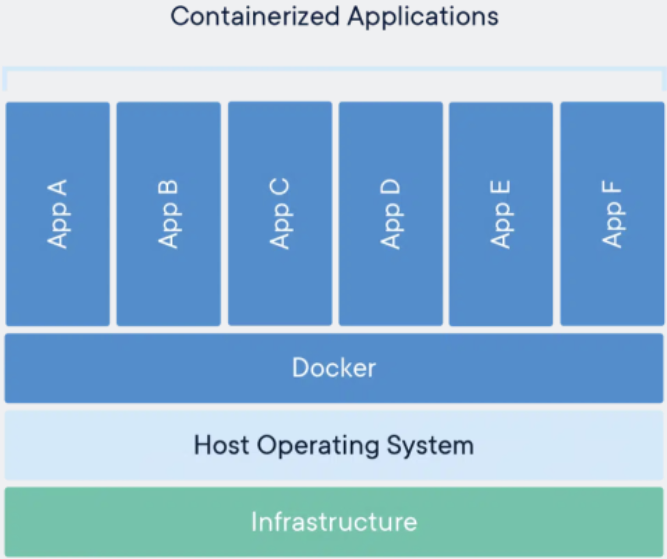
\includegraphics[width=0.7\textwidth]{images/chapter3/docker-containerized-applictions.png}
  \captionsetup{justification=centering}
  \captionsource{Βασική δομή \emph{Dokcer}}{\url{https://www.docker.com/resources/what-container}}
  \label{fig:docker-containers}
\end{figure}
\noindent